%%%%%%%%%%%%%%%%%%%%%%%%%%%%%%%%%%%%%%%%%%%%%%%%%%%%%%%%%%%%%%%%%%%%%%%%%%
%
% 	Template for seminar reports
%
%%%%%%%%%%%%%%%%%%%%%%%%%%%%%%%%%%%%%%%%%%%%%%%%%%%%%%%%%%%%%%%%%%%%%%%%%%

%%%%%%%%%%%%%%%%%%%%%%%%%%%%%%%%%%%%%%%%%%%%%%%%%%%%%%%%%%%%%%%%%%%%%%%%%%
% 	Include layout and macros
%%%%%%%%%%%%%%%%%%%%%%%%%%%%%%%%%%%%%%%%%%%%%%%%%%%%%%%%%%%%%%%%%%%%%%%%%%


%% This LaTeX template is based on the following example file included in the ieeetran
%% package:
%% bare_conf.tex 
%% V1.2
%% 2002/11/18
%% by Michael Shell
%% mshell@ece.gatech.edu
%% (requires IEEEtran.cls version 1.6b or later) with an IEEE conference paper.


% Note that the a4paper option is mainly intended so that authors in
% countries using A4 can easily print to A4 and see how their papers will
% look in print. Authors are encouraged to use U.S. letter paper when 
% submitting to IEEE. Use the testflow package mentioned above to verify
% correct handling of both paper sizes by the author's LaTeX system.
%
% Also note that the "draftcls" or "draftclsnofoot", not "draft", option
% should be used if it is desired that the figures are to be displayed in
% draft mode.
%
% This paper can be formatted using the peerreviewca
% (instead of conference) mode.
\documentclass[conference, a4paper]{IEEEtran-modified}
% If the IEEEtran.cls has not been installed into the LaTeX system files, 
% manually specify the path to it:
% \documentclass[conference]{../sty/IEEEtran} 

\IEEEoverridecommandlockouts

% some very useful LaTeX packages include:

\usepackage{cite}       % Written by Donald Arseneau
                        % V1.6 and later of IEEEtran pre-defines the format
                        % of the cite.sty package \cite{} output to follow
                        % that of IEEE. Loading the cite package will
                        % result in citation numbers being automatically
                        % sorted and properly "ranged". i.e.,
                        % [1], [9], [2], [7], [5], [6]
                        % (without using cite.sty)
                        % will become:
                        % [1], [2], [5]--[7], [9] (using cite.sty)
                        % cite.sty's \cite will automatically add leading
                        % space, if needed. Use cite.sty's noadjust option
                        % (cite.sty V3.8 and later) if you want to turn this
                        % off. cite.sty is already installed on most LaTeX
                        % systems. The latest version can be obtained at:
                        % http://www.ctan.org/tex-archive/macros/latex/contrib/supported/cite/

%\usepackage{graphicx}  % Written by David Carlisle and Sebastian Rahtz
                        % Required if you want graphics, photos, etc.
                        % graphicx.sty is already installed on most LaTeX
                        % systems. The latest version and documentation can
                        % be obtained at:
                        % http://www.ctan.org/tex-archive/macros/latex/required/graphics/
                        % Another good source of documentation is "Using
                        % Imported Graphics in LaTeX2e" by Keith Reckdahl
                        % which can be found as esplatex.ps and epslatex.pdf
                        % at: http://www.ctan.org/tex-archive/info/
% NOTE: for dual use with latex and pdflatex, instead load graphicx like:
\ifx\pdfoutput\undefined
	\usepackage{graphicx}
\else
	\usepackage[pdftex]{graphicx}
\fi

% However, be warned that pdflatex will require graphics to be in PDF
% (not EPS) format and will preclude the use of PostScript based LaTeX
% packages such as psfrag.sty and pstricks.sty. IEEE conferences typically
% allow PDF graphics (and hence pdfLaTeX). However, IEEE journals do not
% (yet) allow image formats other than EPS or TIFF. Therefore, authors of
% journal papers should use traditional LaTeX with EPS graphics.
%
% The path(s) to the graphics files can also be declared: e.g.,
% \graphicspath{{../eps/}{../ps/}}
% if the graphics files are not located in the same directory as the
% .tex file. This can be done in each branch of the conditional above
% (after graphicx is loaded) to handle the EPS and PDF cases separately.
% In this way, full path information will not have to be specified in
% each \includegraphics command.
%
% Note that, when switching from latex to pdflatex and vice-versa, the new
% compiler will have to be run twice to clear some warnings.
\graphicspath{{figures/}}


%\usepackage{psfrag}    % Written by Craig Barratt, Michael C. Grant,
                        % and David Carlisle
                        % This package allows you to substitute LaTeX
                        % commands for text in imported EPS graphic files.
                        % In this way, LaTeX symbols can be placed into
                        % graphics that have been generated by other
                        % applications. You must use latex->dvips->ps2pdf
                        % workflow (not direct pdf output from pdflatex) if
                        % you wish to use this capability because it works
                        % via some PostScript tricks. Alternatively, the
                        % graphics could be processed as separate files via
                        % psfrag and dvips, then converted to PDF for
                        % inclusion in the main file which uses pdflatex.
                        % Docs are in "The PSfrag System" by Michael C. Grant
                        % and David Carlisle. There is also some information 
                        % about using psfrag in "Using Imported Graphics in
                        % LaTeX2e" by Keith Reckdahl which documents the
                        % graphicx package (see above). The psfrag package
                        % and documentation can be obtained at:
                        % http://www.ctan.org/tex-archive/macros/latex/contrib/supported/psfrag/

%\usepackage{subfigure} % Written by Steven Douglas Cochran
                        % This package makes it easy to put subfigures
                        % in your figures. i.e., "figure 1a and 1b"
                        % Docs are in "Using Imported Graphics in LaTeX2e"
                        % by Keith Reckdahl which also documents the graphicx
                        % package (see above). subfigure.sty is already
                        % installed on most LaTeX systems. The latest version
                        % and documentation can be obtained at:
                        % http://www.ctan.org/tex-archive/macros/latex/contrib/supported/subfigure/

\usepackage{url}       % Written by Donald Arseneau
                        % Provides better support for handling and breaking
                        % URLs. url.sty is already installed on most LaTeX
                        % systems. The latest version can be obtained at:
                        % http://www.ctan.org/tex-archive/macros/latex/contrib/other/misc/
                        % Read the url.sty source comments for usage information.

%\usepackage{stfloats}  % Written by Sigitas Tolusis
                        % Gives LaTeX2e the ability to do double column
                        % floats at the bottom of the page as well as the top.
                        % (e.g., "\begin{figure*}[!b]" is not normally
                        % possible in LaTeX2e). This is an invasive package
                        % which rewrites many portions of the LaTeX2e output
                        % routines. It may not work with other packages that
                        % modify the LaTeX2e output routine and/or with other
                        % versions of LaTeX. The latest version and
                        % documentation can be obtained at:
                        % http://www.ctan.org/tex-archive/macros/latex/contrib/supported/sttools/
                        % Documentation is contained in the stfloats.sty
                        % comments as well as in the presfull.pdf file.
                        % Do not use the stfloats baselinefloat ability as
                        % IEEE does not allow \baselineskip to stretch.
                        % Authors submitting work to the IEEE should note
                        % that IEEE rarely uses double column equations and
                        % that authors should try to avoid such use.
                        % Do not be tempted to use the cuted.sty or
                        % midfloat.sty package (by the same author) as IEEE
                        % does not format its papers in such ways.

\usepackage{amsmath}    % From the American Mathematical Society
\usepackage{amssymb}
                        % A popular package that provides many helpful commands
                        % for dealing with mathematics. Note that the AMSmath
                        % package sets \interdisplaylinepenalty to 10000 thus
                        % preventing page breaks from occurring within multiline
                        % equations. Use:
\interdisplaylinepenalty=2500
                        % after loading amsmath to restore such page breaks
                        % as IEEEtran.cls normally does. amsmath.sty is already
                        % installed on most LaTeX systems. The latest version
                        % and documentation can be obtained at:
                        % http://www.ctan.org/tex-archive/macros/latex/required/amslatex/math/

%My packages
\usepackage{todonotes}
\usepackage{pgfplots}
\usepackage{bm}
\usepackage{soul}
\usepackage{lipsum}
\usepackage{verbatim}
\DeclareMathOperator{\sign}{sign}
\DeclareMathOperator{\softmax}{softmax}
\newcommand{\nth}[1]{$#1^\text{th}$}
% \relpenalty=9999

% Other popular packages for formatting tables and equations include:

%\usepackage{array}
% Frank Mittelbach's and David Carlisle's array.sty which improves the
% LaTeX2e array and tabular environments to provide better appearances and
% additional user controls. array.sty is already installed on most systems.
% The latest version and documentation can be obtained at:
% http://www.ctan.org/tex-archive/macros/latex/required/tools/

% Mark Wooding's extremely powerful MDW tools, especially mdwmath.sty and
% mdwtab.sty which are used to format equations and tables, respectively.
% The MDWtools set is already installed on most LaTeX systems. The lastest
% version and documentation is available at:
% http://www.ctan.org/tex-archive/macros/latex/contrib/supported/mdwtools/


% V1.6 of IEEEtran contains the IEEEeqnarray family of commands that can
% be used to generate multiline equations as well as matrices, tables, etc.


% Also of notable interest:

% Scott Pakin's eqparbox package for creating (automatically sized) equal
% width boxes. Available:
% http://www.ctan.org/tex-archive/macros/latex/contrib/supported/eqparbox/



% Notes on hyperref:
% IEEEtran.cls attempts to be compliant with the hyperref package, written
% by Heiko Oberdiek and Sebastian Rahtz, which provides hyperlinks within
% a document as well as an index for PDF files (produced via pdflatex).
% However, it is a tad difficult to properly interface LaTeX classes and
% packages with this (necessarily) complex and invasive package. It is
% recommended that hyperref not be used for work that is to be submitted
% to the IEEE. Users who wish to use hyperref *must* ensure that their
% hyperref version is 6.72u or later *and* IEEEtran.cls is version 1.6b 
% or later. The latest version of hyperref can be obtained at:
%
% http://www.ctan.org/tex-archive/macros/latex/contrib/supported/hyperref/
%
% Also, be aware that cite.sty (as of version 3.9, 11/2001) and hyperref.sty
% (as of version 6.72t, 2002/07/25) do not work optimally together.
% To mediate the differences between these two packages, IEEEtran.cls, as
% of v1.6b, predefines a command that fools hyperref into thinking that
% the natbib package is being used - causing it not to modify the existing
% citation commands, and allowing cite.sty to operate as normal. However,
% as a result, citation numbers will not be hyperlinked. Another side effect
% of this approach is that the natbib.sty package will not properly load
% under IEEEtran.cls. However, current versions of natbib are not capable
% of compressing and sorting citation numbers in IEEE's style - so this
% should not be an issue. If, for some strange reason, the user wants to
% load natbib.sty under IEEEtran.cls, the following code must be placed
% before natbib.sty can be loaded:
%
% \makeatletter
% \let\NAT@parse\undefined
% \makeatother
%
% Hyperref should be loaded differently depending on whether pdflatex
% or traditional latex is being used:
%
%\ifx\pdfoutput\undefined
%\usepackage[hypertex]{hyperref}
%\else
%\usepackage[pdftex,hypertexnames=false]{hyperref}
%\fi
%
% Pdflatex produces superior hyperref results and is the recommended
% compiler for such use.



% *** Do not adjust lengths that control margins, column widths, etc. ***
% *** Do not use packages that alter fonts (such as pslatex).         ***
% There should be no need to do such things with IEEEtran.cls V1.6 and later.


%%%%%%%%%%%%%%%%%%%%%%%%%%%%%%%%%%%%%%%%%%%%%%%%%%%%%%%%%%%%%%%%%%%%%%%%%%
% 	Anpassung an deutsche Texte
%%%%%%%%%%%%%%%%%%%%%%%%%%%%%%%%%%%%%%%%%%%%%%%%%%%%%%%%%%%%%%%%%%%%%%%%%%

%\usepackage{ngerman}
\usepackage[latin1]{inputenc}   % f�r Umlaute 

%\renewcommand{\abstractname}{Kurzfassung}      % statt Zusammenfassung, wie es ngerman definiert
%\renewcommand{\keywordname}{Schl�sselworte}
%\renewcommand{\figurename}{Abb.}




%%%%%%%%%%%%%%%%%%%%%%%%%%%%%%%%%%%%%%%%%%%%%%%%%%%%%%%%%%%%%%%%%%%%%%%%%%
% 	Page numbering (not on first page)
%%%%%%%%%%%%%%%%%%%%%%%%%%%%%%%%%%%%%%%%%%%%%%%%%%%%%%%%%%%%%%%%%%%%%%%%%%
\pagestyle{empty}

%%%%%%%%%%%%%%%%%%%%%%%%%%%%%%%%%%%%%%%%%%%%%%%%%%%%%%%%%%%%%%%%%%%%%%%%%%
% 	Correct bad hyphenation here
%%%%%%%%%%%%%%%%%%%%%%%%%%%%%%%%%%%%%%%%%%%%%%%%%%%%%%%%%%%%%%%%%%%%%%%%%%

\hyphenation{}

%%%%%%%%%%%%%%%%%%%%%%%%%%%%%%%%%%%%%%%%%%%%%%%%%%%%%%%%%%%%%%%%%%%%%%%%%%
% 	Begin of the document
%%%%%%%%%%%%%%%%%%%%%%%%%%%%%%%%%%%%%%%%%%%%%%%%%%%%%%%%%%%%%%%%%%%%%%%%%%

\begin{document}

%%%%%%%%%%%%%%%%%%%%%%%%%%%%%%%%%%%%%%%%%%%%%%%%%%%%%%%%%%%%%%%%%%%%%%%%%%
% 	Paper title
%%%%%%%%%%%%%%%%%%%%%%%%%%%%%%%%%%%%%%%%%%%%%%%%%%%%%%%%%%%%%%%%%%%%%%%%%%

\title{Fundamentals of Neural Networks}

%%%%%%%%%%%%%%%%%%%%%%%%%%%%%%%%%%%%%%%%%%%%%%%%%%%%%%%%%%%%%%%%%%%%%%%%%%
% 	Author names and affiliations 
%		-	multiple columns for up to three different affilitations are separated 
%			by \and
%		- for over three affiliations, refer to ieeetran howto
%%%%%%%%%%%%%%%%%%%%%%%%%%%%%%%%%%%%%%%%%%%%%%%%%%%%%%%%%%%%%%%%%%%%%%%%%%

\author{
\authorblockN{Mathias Jackermeier}
\authorblockA{Fakult�t f�r Informatik\\Technische Universit�t M�nchen\\
Email: mathias.jackermeier@tum.de} 
%\and
%\authorblockN{}
%\authorblockA{}
}

%%%%%%%%%%%%%%%%%%%%%%%%%%%%%%%%%%%%%%%%%%%%%%%%%%%%%%%%%%%%%%%%%%%%%%%%%%
% 	Special paper note (appears between title and authors) 
%%%%%%%%%%%%%%%%%%%%%%%%%%%%%%%%%%%%%%%%%%%%%%%%%%%%%%%%%%%%%%%%%%%%%%%%%%

\specialpapernotice{Seminar Data Mining}

%%%%%%%%%%%%%%%%%%%%%%%%%%%%%%%%%%%%%%%%%%%%%%%%%%%%%%%%%%%%%%%%%%%%%%%%%%
% 	Make title area 
%%%%%%%%%%%%%%%%%%%%%%%%%%%%%%%%%%%%%%%%%%%%%%%%%%%%%%%%%%%%%%%%%%%%%%%%%%

\maketitle

%%%%%%%%%%%%%%%%%%%%%%%%%%%%%%%%%%%%%%%%%%%%%%%%%%%%%%%%%%%%%%%%%%%%%%%%%%
% 	For page number on first page
%%%%%%%%%%%%%%%%%%%%%%%%%%%%%%%%%%%%%%%%%%%%%%%%%%%%%%%%%%%%%%%%%%%%%%%%%%

%\thispagestyle{plain}

%%%%%%%%%%%%%%%%%%%%%%%%%%%%%%%%%%%%%%%%%%%%%%%%%%%%%%%%%%%%%%%%%%%%%%%%%%
% 	Abstract 
%%%%%%%%%%%%%%%%%%%%%%%%%%%%%%%%%%%%%%%%%%%%%%%%%%%%%%%%%%%%%%%%%%%%%%%%%%

\begin{abstract}
Neural networks are biologically inspired computation models that have shaped the field of machine learning over the last decade, enabling breakthroughs in numerous application areas ranging from image processing to natural language understanding. In this paper, we review the fundamental principles behind neural networks, providing the reader with the necessary mathematical knowledge to be able to use them in practice. We examine the development of neural networks from simpler models, their architecture and related design decisions, and their mathematical specification. We then explore the most common training algorithm employed in neural networks. Finally, we briefly discuss more advanced network architectures and the continued impact we believe neural networks will have on machine learning.
\end{abstract}


%%%%%%%%%%%%%%%%%%%%%%%%%%%%%%%%%%%%%%%%%%%%%%%%%%%%%%%%%%%%%%%%%%%%%%%%%%
% 	Keywords 
%%%%%%%%%%%%%%%%%%%%%%%%%%%%%%%%%%%%%%%%%%%%%%%%%%%%%%%%%%%%%%%%%%%%%%%%%%

\begin{keywords}
test
\end{keywords}


%%%%%%%%%%%%%%%%%%%%%%%%%%%%%%%%%%%%%%%%%%%%%%%%%%%%%%%%%%%%%%%%%%%%%%%%%%
% 	Sections, Subsections,...
%%%%%%%%%%%%%%%%%%%%%%%%%%%%%%%%%%%%%%%%%%%%%%%%%%%%%%%%%%%%%%%%%%%%%%%%%%

\section{Introduction}
Artificial intelligence systems have been becoming more and more powerful over the last 10 years. We have seen outstanding advances in a variety of fields including computer vision, natural language processing and fraud detection, which power many end-user technologies such as digital assistants or self-driving cars. Much of the recent progress can be attributed to \emph{deep learning}, a powerful set of techniques that enable computers to understand the world by decomposing complex concepts into a hierarchy of simpler abstractions.

While numerous other approaches to machine learning exist, deep learning has shown to outperform other methods in a wide variety of applications. To name a few examples, deep learning models dominate the task of object recognition in images \cite{DBLP:journals/ijcv/RussakovskyDSKS15}, even surpassing human-level performance \cite{DBLP:conf/iccv/HeZRS15}, have been successfully applied to sentiment analysis \cite{DBLP:conf/sigir/SeverynM15a}, and
have significantly improved speech recognition systems \cite{DBLP:journals/taslp/MohamedDH12}. Deep learning has also been used in problems such as style transfer between images \cite{DBLP:conf/cvpr/GatysEB16}, image description generation \cite{DBLP:journals/pami/KarpathyF17}, and learning to play video games \cite{DBLP:journals/nature/MnihKSRVBGRFOPB15}.

By learning everything required to solve a task purely from raw data, these techniques have alleviated the need for problem-specific expert knowledge. Thus, very similar models building on the same core ideas can be applied to a vast array of different tasks with outstanding success.

One such core idea that is fundamental to deep learning is the \emph{neural network}, a computing model loosely inspired by neuroscience. While neural networks are not new, it was not until recently that enough data and computational resources became available to train them effectively and fully appreciate their power \cite[Ch.\,1,\,pp.\,18-21]{DBLP:books/daglib/0040158}.

Since neural networks have become so prevalent in modern machine learning applications, many libraries exist that abstract their concepts and provide simple programming interfaces. However, it does not suffice to be familiar with such libraries to use neural networks effectively; in order to understand which architectures perform well, and why, one must also know their mathematical foundations.

In this paper we thus aim to give a thorough overview of neural networks and the fundamental techniques and algorithms associated with them. We first briefly examine the motivation and history behind neural networks in Section \ref{sec:perceptron} by introducing the \emph{perceptron} model. Section \ref{sec:feedforward_neural_networks} then shows how this model has been adjusted and extended to obtain the neural network, focusing in particular on \emph{feedforward neural networks}. We also discuss several design choices that have to be taken into account when working with these models. In Section \ref{sec:training}, we explain how these networks can be trained, introducing ideas such as \emph{stochastic gradient descent} and \emph{back-propagation}. Section \ref{sec:extensions} briefly examines extensions of feedforward neural networks that are commonly used in practice, before we conclude our paper in Section \ref{sec:conclusion}.
\section{The Perceptron}
\label{sec:perceptron}
When researchers developed the first machine learning models, they often used ideas based closely on our understanding of the brain. One such model, inspired by the biological neuron, is the perceptron, which was first conceived by \cite{McCulloch1943115}.

Like its biological counterpart, the perceptron receives information and produces an output. More specifically, it accepts $n$ input values $x_1, \ldots, x_n$ and calculates a corresponding output value $\hat{y} \in \{-1, 1\}$ by computing
\begin{equation}\label{eq:perceptron1}
	\hat{y} = \text{sign}\left (\sum_{i=1}^{n} w_ix_i\right ),
\end{equation}
where the weights $w_i$ are the parameters of the model, and $\text{sign}(x)$ is defined as
\begin{equation}
\text{sign}(x) = \begin{cases} 1 & \text{if }x \geq 0
							\\-1 & \text{if }x < 0.
\end{cases}
\end{equation}
By representing the input values and weights as vectors $\bm{x}$ and $\bm{w}$, we can rewrite \eqref{eq:perceptron1} as
\begin{equation}
\hat{y} = \text{sign}(\bm{w}^\top\bm{x}).
\end{equation}
For a visual representation of this model, see Fig. \ref{fig:perceptron}. 

\begin{figure}
	\begin{center}
		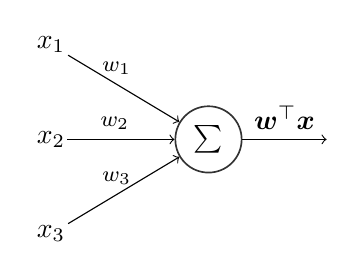
\begin{tikzpicture}
	\tikzstyle{neuron} = [circle,draw=black!80,semithick,minimum size=20pt]
	% input layer
	\foreach \i in {1,...,3}
		\node (input\i) at (0, -\i*1.2) {$x_\i$};
	% perceptron
	\node[neuron] (perceptron) at (2, -2*1.2) {$\sum$};
	% connections
	\foreach \i in {1,...,3}
		\draw[->, shorten <= -.1cm] (input\i) -- node[pos=.4,above]{\footnotesize{$w_\i$}} (perceptron);
	% output
	\draw[->] (perceptron) -- node[above]{$\bm{w}^{\top}\bm{x}$}(3.5, -2*1.2);
\end{tikzpicture}
	\end{center}
	\caption{An illustration of the perceptron model. In this example, the perceptron accepts three inputs $x_1, x_2, x_3$, has the parameters $w_1, w_2, w_3$, and computes $\hat{y} = \text{sign}(w_1x_1 + w_2x_2 + w_3x_3).$}
	\label{fig:perceptron}
\end{figure}

Perceptron models can be used to solve binary classification problems. In this scenario, we are given a set of $m$ training examples $\mathbb{X} = \{\bm{x}^{(1)}, \ldots, \bm{x}^{(m)}\}$ and their corresponding binary labels $\mathbb{Y}$, and wish to predict the most probable label for an unseen vector $\bm{x} \notin \mathbb{X}$.

For example, the vectors $\bm{x}^{(i)}$ might describe features of an email using a \emph{bag-of-words} representation. That is, we define a fixed vocabulary, and the $j$th entry in the vector $\bm{x}^{(i)}$ specifies how often the $j$th word of the vocabulary occurs in the particular email represented by $\bm{x}^{(i)}$. The corresponding label $y^{(i)} = 1$ then might signify that the email is a legitimate email, whereas a value of $y^{(i)} = -1$ might label the email as spam.

In the beginning, the weights are randomly initialized and the model thus makes arbitrary predictions. During the process of \emph{training} the perceptron, we iteratively adjust the weights in order to improve the prediction accuracy on the training set.

One common method of training is the perceptron learning algorithm proposed by \cite{Rosenblatt1958386}. Essentially, the algorithm iterates through the training data $\mathbb{X}$ and makes small adjustments to the weights if a particular training example $x^{(i)}$ is misclassified. For example, if the perceptron predicts $\hat{y} = 1$ and the actual label is $y^{(i)} = -1$, the weights are corrected in the negative direction. Since the perceptron learning algorithm is not directly applicable to neural networks, we will not discuss it further; a more in depth explanation can be found in \cite[Ch.\,8,\,pp.\,265-267]{DBLP:books/lib/Murphy12}.

A major shortcoming of the perceptron is that it can only learn to classify linearly separable data \cite{DBLP:books/daglib/0066902}. For example, the \textsc{xor} function, where 
\begin{equation}
\text{\textsc{xor}}(x) = 
\begin{cases} 0 & \text{if }x = [0,0] \lor x = [1,1] 
			\\1 & \text{if }x = [1,0] \lor x = [0,1],
\end{cases}
\end{equation}
cannot be learned with the perceptron. The discovery of these limitations has greatly reduced interest in the field of biological learning, until more sophisticated models, such as neural networks, were developed \cite[Ch.\,1,\,pp.\,12-18]{DBLP:books/daglib/0040158}.
\section{Feedforward Neural Networks}
\label{sec:feedforward_neural_networks}
\section{Training Feedforward Neural Networks}
\label{sec:training}
\section{Universal Approximation Capabilities}
\label{sec:approximation}

%\section{Extensions and Applications}
\label{sec:extensions}
\section{Conclusion}
\label{sec:conclusion}
We have discussed feedforward neural networks, a biologically inspired computing model that dominates modern machine learning. Feedforward neural networks are complex networks of simple units which are arranged in a layered architecture. By propagating an input through its layers, a neural network can make sophisticated predictions, such as which class the input is most likely to belong to.

Neural networks can be represented as a chain of matrix operations and applications of nonlinear functions. The parameters of the model are chosen during training, where a cost function that measures the performance of the network is minimized. The most common algorithm to achieve this is stochastic gradient descent, which requires the computation of the gradient of the cost function. This is efficiently handled by the back-propagation algorithm.

\begin{comment}
Deep learning, the branch of machine learning that is concerned with the development of deep neural networks, has enabled an outstanding amount of advances in the field. 
\end{comment}
We believe that, with ever-increasing datasets and computational power, as well as the development of more complex and refined models, neural networks will continue to have a great impact on technology and will power more and more intelligent systems in the future.

%%%%%%%%%%%%%%%%%%%%%%%%%%%%%%%%%%%%%%%%%%%%%%%%%%%%%%%%%%%%%%%%%%%%%%%%%%
% 	Acknowledgements
%%%%%%%%%%%%%%%%%%%%%%%%%%%%%%%%%%%%%%%%%%%%%%%%%%%%%%%%%%%%%%%%%%%%%%%%%%

%\section*{Acknowledgment}
%\addcontentsline{toc}{section}{Acknowledgment}

%%%%%%%%%%%%%%%%%%%%%%%%%%%%%%%%%%%%%%%%%%%%%%%%%%%%%%%%%%%%%%%%%%%%%%%%%%
% 	References
%%%%%%%%%%%%%%%%%%%%%%%%%%%%%%%%%%%%%%%%%%%%%%%%%%%%%%%%%%%%%%%%%%%%%%%%%%

% trigger a \newpage just before the given reference
% number - used to balance the columns on the last page
% adjust value as needed - may need to be readjusted if
% the document is modified later
%\IEEEtriggeratref{8}
% The "triggered" command can be changed if desired:
%\IEEEtriggercmd{\enlargethispage{-5in}}

% references section
% NOTE: BibTeX documentation can be easily obtained at:
% http://www.ctan.org/tex-archive/biblio/bibtex/contrib/doc/

% can use a bibliography generated by BibTeX as a .bbl file
% standard IEEE bibliography style from:
% http://www.ctan.org/tex-archive/macros/latex/contrib/supported/IEEEtran/bibtex
\bibliographystyle{IEEEtran}
% argument is your BibTeX string definitions and bibliography database(s)
\bibliography{jabref}
%
% <OR> manually copy in the resultant .bbl file
% set second argument of \begin to the number of references
% (used to reserve space for the reference number labels box)
%\begin{thebibliography}{1}
%
%\bibitem{ref:kopka}
%H.~Kopka and P.~W. Daly, \emph{A Guide to {\LaTeX}}, 3rd~ed.\hskip 1em plus
%  0.5em minus 0.4em\relax Harlow, England: Addison-Wesley, 1999.
%
%\end{thebibliography}

%%%%%%%%%%%%%%%%%%%%%%%%%%%%%%%%%%%%%%%%%%%%%%%%%%%%%%%%%%%%%%%%%%%%%%%%%%
% 	End of the document
%%%%%%%%%%%%%%%%%%%%%%%%%%%%%%%%%%%%%%%%%%%%%%%%%%%%%%%%%%%%%%%%%%%%%%%%%%

\end{document}


